%% ------------------------------------------------------------------------- %%
\chapter{Introdução}
\label{cap:introducao}

Test-Driven Development (TDD) é uma das práticas discutidas pela Programação
Extrema (XP) \cite{XPExplained}. A prática é baseada em um pequeno ciclo de
desenvolvimento, na qual o desenvolvedor deve sempre escrever um teste antes
mesmo de implementar a funcionalidade esperada, e depois, com o novo teste
passando, o desenvolvedor deve refatorar para remover duplicação
\cite{TDDByExample}.
Mas, apesar da constante escrita de testes automatizados, os benefícios da
prática vão além disso. Na opinião de muitos autores conhecidos, TDD promove
uma melhoria significativa no design de classes, auxiliando o programador a
criar classes mais coesas e menos acopladas \cite{TDDByExample} \cite{GOOS} 
\cite{astels-tdd}.

Discutir os efeitos de TDD no design de classes é de grande importância para os
desenvolvedores.
Criar classes ou, em um nível maior de abstração, módulos que possuam um baixo
acoplamento e uma alta coesão demandam um esforço muito grande do desenvolvedor. 
É muito comum que, após algum tempo de desenvolvimento, o design perca qualidade
e qualquer tipo de manutenção torne-se difícil e, por consequência, custosa.
Muitas práticas tentam reduzir esses problemas, como programação pareada ou
revisão de código. Os praticantes de TDD acreditam que os testes sejam uma outra
maneira de validar o design criado, e utilizar esse feedback para melhorá-lo.

É possível observar a crescente adoção e procura por TDD
através do número de pesquisas publicadas pela academia.
Em um questionário de 2010 para descobrir que práticas eram feitas por times
ágeis \cite{wambler-survey-agile}, Scott Ambler mostrou que 53\% dos times ágeis
adotaram TDD como uma maneira para validar o trabalho feito, conforme mostra a 
Figura \ref{fig:wambler-agile-2010}. Outro questionário de 2008 também realizado por Ambler
\cite{wambler-survey-tdd}, focado em TDD, mostra que 57\% dos desenvolvedores 
utilizam TDD como técnica para capturar informações de design, conforme mostrado
na Figura \ref{fig:wambler-tdd-2008}.

No Brasil, é possível observar o crescente número de pessoas atrás de
informações sobre a prática nas mais diversas listas de discussão e fóruns sobre
tecnologia, como o GUJ \footnote{\url{http://www.guj.com.br}.
Último acesso em 27 de fevereiro 2011} ou o .NET Architects 
\footnote{\url{http://www.dotnetarchitects.net/}. Último acesso em
27 de fevereiro de 2011}. Diversos eventos de desenvolvimento de
software realizados no Brasil em 2010, como a QCON SP
\footnote{\url{http://www.qconsp.com/}. Último acesso em 02 de março de 2011} e
a Agile Brazil \footnote{\url{http://http://www.agilebrazil.com/}. Último acesso
em 02 de março de 2011} também contaram com palestras sobre o assunto.

Os aficionados por TDD dizem que estão \textit{``infectados pelo teste''}  e,
segundo eles próprios, desenvolvedores que experimentam a prática e percebem
seus efeitos tendem a não voltar atrás \cite{tdd-fearless}.
Já Robert Martin relaciona TDD à profissionalismo. Segundo ele, um desenvolvedor
profissional entrega código claro e flexível que funcione dentro do prazo, e TDD
possibilita que o desenvolvedor alcance esses pontos \cite{martin-profissionalismo}.

Entretanto, grande parte dos experimentos feitos pela academia verificam os
efeitos da prática sobre a qualidade externa. Poucos são os estudos que avaliam TDD do
ponto de vista da qualidade interna de código. Muitos desses estudos
inclusive são feitos em laboratórios, diminuindo o realismo do experimento. 
Siniaalto e Abrahamsson também
compartilham dessa opinião e, além disso, notaram que os efeitos de TDD podem 
não ser tão automáticos ou evidentes como o esperado \cite{alarming-results}.
Este trabalho visa compreender os efeitos e como a prática de TDD
influencia no design de sistemas orientados a objetos do ponto de vista dos
desenvolvedores que a praticam.

Mas conduzir uma pesquisa no mundo real implica em um equilíbrio entre
nível de controle e grau de realismo. Uma situação realística é geralmente complexa e 
não-determinística, impedindo o entendimento sobre o que acontece. Por outro
lado, aumentar o controle sobre o experimento reduz o grau de realismo, muitos
vezes fazendo com que os reais fatores de influência fiquem fora do escopo do 
estudo. Estudos de caso são, por definição, conduzidos no mundo real e por isso 
têm um alto grau de realismo, mas dessa forma sacrificando o nível de  controle
\cite{guidelines-case-study}.
Baseando-se no fato de que o processo de desenvolvimento de software envolve 
diversos fatores humanos e é totalmente sensível ao contexto em que ele está 
inserido, este trabalho é composto por um conjunto de estudos de caso em
empresas do mercado brasileiro de software, que já utilizam TDD normalmente
dentro do seu ciclo de desenvolvimento. Os métodos de pesquisa utilizados por
esse trabalho são melhor explicados no Capítulo \ref{cap:planejamento}.

\begin{figure}[ht]
  \begin{minipage}[b]{0.45\linewidth}
    \centering
    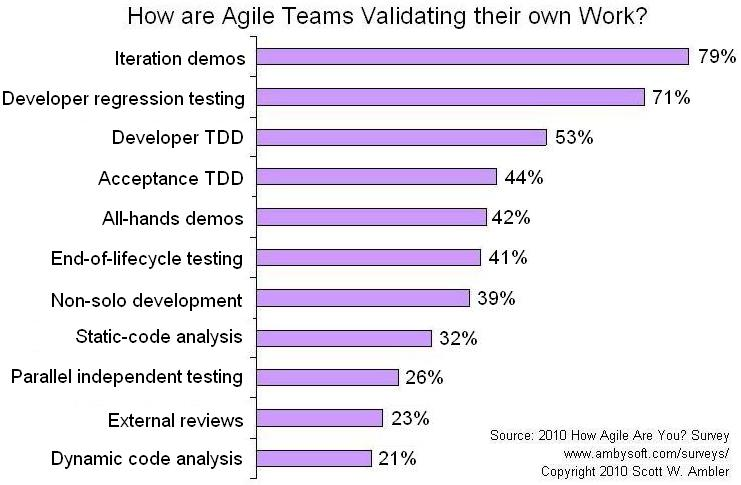
\includegraphics[scale=.4]{agileCriteria2010Validating}
    \caption{Como times ágeis validam seu próprio trabalho?}
    \label{fig:wambler-agile-2010}
  \end{minipage}
  \hspace{0.5cm}
  \begin{minipage}[b]{0.45\linewidth}
    \centering
    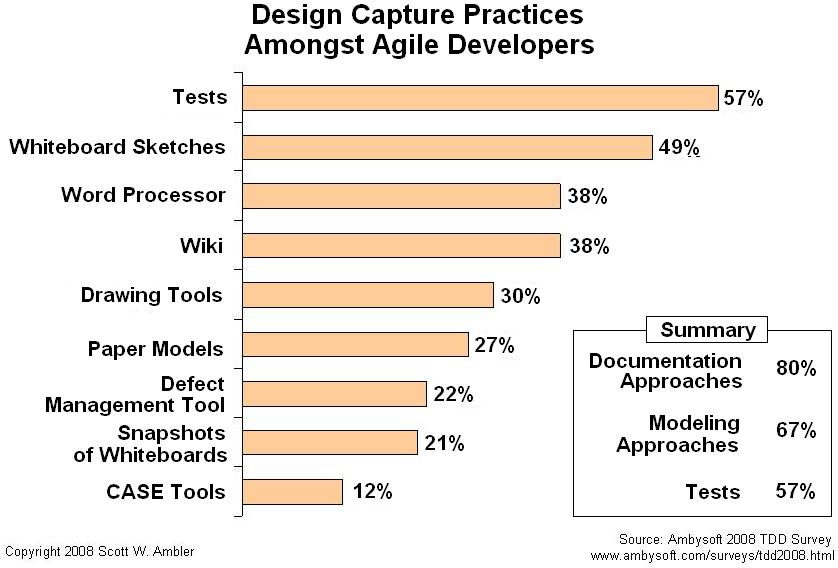
\includegraphics[scale=.35]{tddDesignPractices}
    \caption{Maneiras de captura de design entre desenvolvedores ágeis}  
    \label{fig:wambler-tdd-2008}
  \end{minipage}
\end{figure}			

%% ------------------------------------------------------------------------- %%
\section{Contribuições}

O objetivo desta pesquisa é entender como TDD influencia no design de sistemas
orientados a objetos. A análise será feita através de dados que serão
capturados baseados na percepção de programadores que realizam a prática no seu
dia-a-dia de trabalho.
Os objetivo principal da pesquisa é \textbf{entender a influência de TDD no
design de sistemas orientados a objetos}.

Como mencionado acima, praticantes de TDD afirmam que a prática os ajuda a criar
classes que apresentam simplicidade, baixo acoplamento e alta coesão. Para
compreender esses efeitos, essa pesquisa tenta responder as questões listadas
abaixo:

\begin{enumerate}

  \item Como o teste guia o desenvolvedor durante a atividade de
  design?

  \item Como a prática de TDD afeta o acoplamento das classes criadas?

  \item Como a prática de TDD afeta o gerenciamento de dependências em sistemas
  orientados a objetos?

  \item Como a prática de TDD afeta a coesão das classes criadas?

  \item Como TDD afeta a simplicidade das classes criadas?

\end{enumerate}

%% ------------------------------------------------------------------------- %%
\section{Organização do trabalho}

Este trabalho está dividido da seguinte maneira: 

\begin{itemize}
	\item O Capítulo \ref{cap:tdd} discute sobre a prática de TDD, com ênfase no
	ponto de vista do design.
  
	\item O Capítulo \ref{cap:trabalhos-relacionados} mostra trabalhos já
	realizados pela academia sobre os efeitos de TDD.

 	\item O Capítulo \ref{cap:qualitativo} discute métodos qualitativos de
 	pesquisa e suas características;

	\item O Capítulo \ref{cap:planejamento} discute o planejamento do experimento,
	bem como o processo de captura de dados e análise;

	\item O Capítulo \ref{cap:discussao} apresenta os resultados encontrados e
	discute em cima dos mesmos.
	
	\item O Capítulo \ref{cap:ameacas} discute as possíveis ameaças dos resultados
	encontrados na pesquisa.
	
	\item O Capítulo \ref{cap:conclusoes} resume o trabalho realizado a apresenta
	possibilidades de trabalhos futuros.
\end{itemize}

